\documentclass[border=2pt,tikz]{standalone}
\usepackage{tikz}
\usepackage{amsmath}
\usepackage{amssymb}

\begin{document}

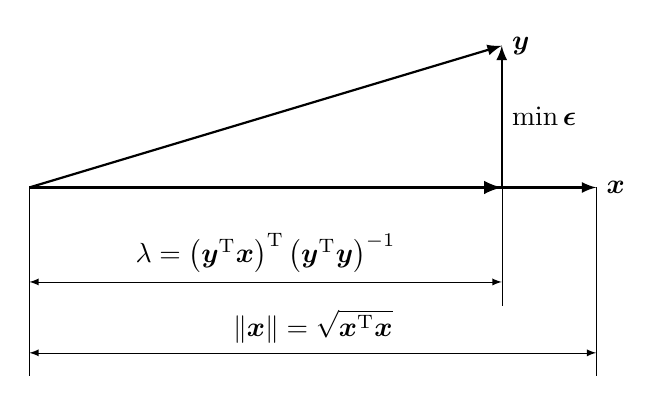
\begin{tikzpicture}[scale=6]

\draw[thick, ->,>=latex] (0.0, 0.0) -- (1.0, 0.3) node [right] {$\boldsymbol{y}$} ;
\draw[thick, ->,>=latex] (1.0, 0.0) -- node [right] {$\min \boldsymbol{\epsilon}$} (1.0, 0.3) ;
\draw[thick, ->,>=latex] (0.0, 0.0) -- (1.2, 0.0) node [right] {$\boldsymbol{x}$} ;

\draw[very thick, ->,>=latex] (0.0, 0.0) -- (1.0, 0.0);
\draw[very thin] (0.0, 0.0) -- (0.0,-0.4) ;
\draw[very thin] (1.0, 0.0) -- (1.0,-0.25) ;
\draw[very thin, <->,>=latex] (0.0,-0.2) -- node [above] {$\lambda=\left(\boldsymbol{y}^{\mathrm{T}}\boldsymbol{x}\right)^{\mathrm{T}}\left(\boldsymbol{y}^{\mathrm{T}}\boldsymbol{y}\right)^{-1}$} (1.0,-0.2);
\draw[very thin] (1.2, 0.0) -- (1.2,-0.4) ;
\draw[very thin, <->,>=latex] (0.0,-0.35) -- node [above] {$\left\Vert \boldsymbol{x}\right\Vert =\sqrt{\boldsymbol{x}^{\mathrm{T}}\boldsymbol{x}}$} (1.2,-0.35);

\end{tikzpicture}

\end{document}

